\section{Lesson 140 CONDICIONALES CON WOULD}

Hi! how's it going?, welcome to lesson 140.\\

In the previous lesson you used the special conditional form
could.\\
En la lección previa usaste la forma condicional especial could.

And you've saw that it's used for all of these forms.\\
Y viste que se usa para todas estas formas.

\begin{verbatim}
You could go on the train.
Tú podrías...
Usted podría...
Vosotros podrían...
Ustedes podrían...
...ir en tren.
\end{verbatim}

But that's a special case.\\
Pero ese es un caso especial.

In the next four lessons I want to show you how we
normally do conditionals with verbs.\\
En las proximas cuatro lecciones quiero mostrarte como normalmente hacemos
las condicionales con los verbos.

We're going to need four lessons.\\
Vamos a necesitar 4 lecciones.

Because we've got to do the long form, the short forms and questions in
positive and negative.\\
Porque tenemos que hacer la forma larga, las formas acortadas más las
preguntas en afirmativo y en negativo.

and that there are some interesting pronunciations to learn.\\
Y hay unas pronunciaciones interesantes para aprender.

In this lessons we're interested in the forms like these in Spanish which
have these endings.\\
En esta lección nos interesan las terminaciones así como estas en español
las cuales tienen estas terminaciones.

hablar\textcolor{yellow}{ía}\\
hablar\textcolor{yellow}{ías}\\
hablar\textcolor{yellow}{ía}\\
hablar\textcolor{yellow}{íamos}\\
hablar\textcolor{yellow}{íais}\\
hablar\textcolor{yellow}{ían}\\

In English, it's really easy to form a basic conditional because we don't
have all of these endings, we just have one word that shows us that it's a
conditional.\\
En inglés es muy fácil formar una condicional básica porque no tenemos
todas estas terminaciones, tenemos solo una palabra que nos muestra que es
una condicional.

It goes in front of the verb.\\
Va delante del verbo.

I \textcolor{yellow}{\_\_\_\_\_} speak.\\
You \textcolor{yellow}{\_\_\_\_\_} speak.\\
He \textcolor{yellow}{\_\_\_\_\_} speak.\\
She \textcolor{yellow}{\_\_\_\_\_} speak.\\
We \textcolor{yellow}{\_\_\_\_\_} speak.\\
They \textcolor{yellow}{\_\_\_\_\_} speak.\\

And that word is "would".\\
Y esa palabra es "would".

\begin{figure}[H]
\centering
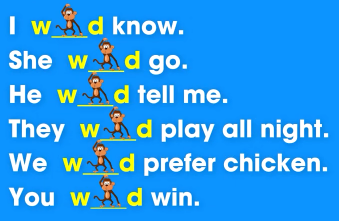
\includegraphics{106.png}
\end{figure}

I would know.\\
Yo sabría.

She would go.\\
Ella iría.

He would tell me.\\
El me lo diría.

They would play all night.\\
Ellos jugarian toda la noche.

We would prefer chicken.\\
Nosotros preferiríamos pollo.

You would win.\\
Tu ganarías.

See instead of endings we've just got this word would.\\
Ves que en vez de terminaciones, nosotros solo tenemos la palabra "would".

It's a if we were saying "you conditional win".\\
Es como si dijeramos "tu condicional ganar".

Es decir "Ganarías tu."

Obviously you've noticed that I've shown the word "would" with a monkey in
the middle instead of letters.\\
Oviamente has notado que he mostrado la palabra "would" con un mono entre
medio en vez de letras.

Why do you think I've done that?.\\
¿Por qué crees que he hecho eso.?

Because when we say "would" we normally use the monkey sound.\\
Porque cuando decimos "Would", normalmente usamos el sonido de mono.

Repeat this magnificent sound.\\
Repite este magnífico sonido.

I've also put the monkey in because the spelling of "would" is a bit strange.\\
Tambien he insertado el mono porque la ortografia de "would" es un poco rara.

What letters do you think we use to make this sound?.\\
¿Que letras crees que usamos para hacer este sonido?.

In this case we use oul.\\
En este caso usamos oul.

\begin{figure}[H]
\centering
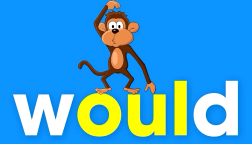
\includegraphics{107.png}
\end{figure}

Don't try to pronounce the L we don't say it.\\
No intentes pronunciar la L, no la decimos.

Nobody.\\
Nadie.

It's wrong.\\
Esta mal.

It's just the monkey sound.\\
es solo el sonido de cavernicola.

Si te sale una g al principio con la pronunciación, simplemente quita la
b de bueno e intenta pronunciarlo.

I've said loads of times that English spelling isn't your friend.\\
He dicho un monton de veces que la ortografia inglesa no es tu amiga.

It's very inconsistent.\\
Es muy inconsistente.

There's also a word "wood" that sounds exactly the same.\\
Hay tambien una palabra "wood" que suena exactamente igual.

\begin{figure}[H]
\centering
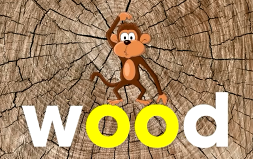
\includegraphics{108.png}
\end{figure}

It's spelt wood.\\
Se deletrea wood.

It means "madera".\\
Quiere decir madera.

So if you hear "W\_\_d" you need to decide if it's a conditional or if it's
wood from a tree.\\
Asi que si escuchas "W\_\_d" tienes que decidir si es una condicional o si
es madera de un arbol.

Let's practice, decide what the following sentences mean.\\
Practiquemos, decide que quieren decir las siguientes oraciones.

John would help.\\
John ayudaría.

Note that you don't put an s on the end of the verb help.\\
Nota que no se pone una s al final del verbo help.

After would we use the infinitive the base form without s.\\
Despues de would usamos el infinitivo la forma base sin s.

Number two.\\
They would prefer to go home.\\
Ellos preferirían ir a casa.

Number three.\\
She would live with you.\\
Ella viviría con tigo.

Nota que no hay ninguna s, would es igual en todos los pronombres personales,
no cambia y despues se pone el infinitivo.

I would wait till later.\\
Yo esperaría hasta más tarde.

Number five.\\
My parents would do it tonight.\\
Mis padres lo harian esta noche.

Number six.\\
He would prefer it with bacon.\\
El lo preferiría con panceta.

Lots of things are better with bacon.\\
Muchas cosas son mejores con panceta.

Now I'm going to make a few mistakes.\\
Ahora voy a unos errores.

Can you see them?.\\
¿Puedes verlos?

Mistake number 1.\\
Error número 1.

Ella sabría.\\
She would\textcolor{yellow}{s} know. \textcolor{red}{$\times$}\\
She would know. \textcolor{green}{\checkmark}

The mistake is the "s" at the end of "would".\\
El error es la "s" al final de "would".

Would is the same in every person.\\
Would es igual en todas las personal.

Mistake number 2.\\
El lo haría.\\
He would do\textcolor{yellow}{es} it. \textcolor{red}{$\times$}\\
He would do it. \textcolor{green}{\checkmark}

Can you see the mistake?.\\
¿Puedes ver el error?.

The mistake is the word "does".\\
El error es la palabra "does".

We use the infinitive after the word "would".\\
Usamos el infinitivo despues de la palabra "would".

No s.\\
Sin s.

Mistake numbre 3.\\
Yo podría hacerlo facilmente.
I would \textcolor{yellow}{can} do it easily.\textcolor{red}{$\times$}\\
I could do it easily.\textcolor{green}{\checkmark}\\
I would be able to do it easily.

Can you remember the spacial conditional form from the previous lesson.\\
¿Te acuerdas la forma condicional especial de la lección anterior?.

In that lesson we used the word "could".\\
En esa lección usamos la palabra "would".

En realidad hay dos opciones, se puede decir "I could do it easily" con
la palabra "could" con la condicional especial, o se puede decir "I would
be able to do it easily".\\

Ambas versiones estan bien, aunque obviamente "could" sería más común siendo
tan corta y tan bonita.

Decir "I would can ..." suena muy mal porque can no tiene infinitivo
y en varios casos tenemos que robar "be able to" porque "can" no tiene
infinitivo en el idioma moderno.

Now it's you turn.\\
Ahora es tu turno.

Let's practice.\\
Practiquemos.

Yo tendría perro.\\
I would have a dog.

Mamá sabría.\\
Mum would know.

Nosotros preferiríamos quedarnos en londres.\\
We would prefer to stay in London.

Yo me fijaría en el garage.\\
I would look in the garage.

El inglesito lo pronuncia garage como "gárech".

Yo pediría más dinero.\\
I would ask for more money.

Si no ponemos la palabra "for", se entiende "ask" como preguntar.

Yo te podría ayudar mañana.\\
I would be able to help you tomorrow.

I could help you tomorrow.

But I told you to say it with would.\\
Pero te dije que lo digas con una sola palabra.

But it's the same thing.\\
Pero es lo mismo.

Very good.\\
Muy bien.

Would tiene dos pronunciaciones, una fuerte que se hace con el sonido de
mono y el sonido débil que es el sonido de cabernicola.

Edward Woodward. es el nombre de un actor famoso en inglaterra.

Podemos hacer le sonido intercambiado de sonido débil y el sonido fuerte
en este nombre de este actor y adicionando la palabra would.

Edward Woodward would.

Edward Woodward was a famous actor.\\
Edward Woodward era un actor famoso.



